\chapter{服务监控与应急措施优化}
在本论文的第三章和第四章分别对应用性能方面和数据库方面进行了优化,在系统优化的过程中,除了提升应用性能和数据库性能这两方面之外,对于服务器中运行的服务进行监控检查和报警,并且能够实现自动化的Failover也是系统优化的重点,本章将对于目前项目开发过程中使用的工具和软件设计开发相应的监控脚本,并且探索在服务监控过程中的报警和故障恢复模式\cite{刘雄辉2007服务器监控管理}。
\label{cha:Monitor}
\section{阿里云云监控应用}
云监控(CloudMonitor)服务是由阿里云推出的,它的目的是对阿里云上的资源和互联网应用进行状态的监控。通过云监控服务,可以根据自定义规则获取阿里云资源的各项监控指标,可以通过设置服务的访问方式来探测服务的可用性,除此之外还可以对监控指标设置报警并及时通知运维人员。由于本项目的所有服务器均为阿里云服务器,所以一部分的监控可以通过配置阿里云资源的监控规则来对部分服务和资源状态进行监控,如对云服务器、云数据库和负载均衡等资源的监控,亦可以实现对使用HTTP和ICMP这些比较通用的网络协议的服务进行监控,保证网络服务的正常运行\cite{梁宇2014基于}。

在正式进行阿里云监控配置前,需要对目前阿里云资源进行统计,如表~\ref{tab:aliyun-resources}所示:

\begin{longtable}[c]{c*{2}{cp{7cm}}}
\caption{项目阿里云资源整理}\label{tab:aliyun-resources}\\
\toprule[1.5pt]
{\heiti 资源类别} & \multicolumn{1}{c}{\heiti 资源实例}  & {\heiti 资源介绍} \\\midrule[1pt]
\endfirsthead
\multicolumn{3}{c}{续表~\thetable\hskip1em 项目阿里云资源整理}\\
\toprule[1.5pt]
{\heiti 资源类别} & \multicolumn{1}{c}{\heiti 资源实例}  & {\heiti 资源介绍} \\\midrule[1pt]
\endhead
\hline
\multicolumn{3}{r}{续下页}
\endfoot
\endlastfoot
\multirow{5}*{站点} &  生产环境地址 & 生产环境应用的负载均衡入口地址  \\
                        &  测试环境地址 & 测试环境应用的负载均衡入口地址  \\
                        &  主数据库地址 & 生产环境主数据库的访问地址和端口  \\
                        &  从数据库地址 & 生产环境从数据库的访问地址和端口  \\
                        &  Couchbase地址  & 生产环境Couchbase入口地址\\
\hline
\multirow{5}*{云服务器ECS}  &  APP1 & WEB应用服务器,提供WEB应用服务  \\
                        &  APP2 & WEB应用服务器,提供WEB应用服务  \\
                        &  DB1 & 主数据库服务器,WEB请求的主服务器  \\
                        &  DB2 & 从数据库服务器,同DB1主从复制,DB1出现问题时切换为主数据库  \\
                        &  TEST & 测试服务器,提供测试环境相关的服务  \\
\hline
\multirow{3}*{负载均衡}  &  prod & 生产环境WEB应用负载均衡  \\
                        &  dbslb & 生产环境数据库负载均衡  \\
                        &  test & 测试环境负载均衡  \\
\multirow{3}*{CDN}  &  web & WEB应用访问域名  \\
                    &  img & 图片服务器域名  \\
                    &  fileserver & 文档服务器域名  \\
\bottomrule[1.5pt]
\end{longtable}

为了保证各个阿里云资源的正常使用,通过阿里云的云监控配置各服务的监控项,并且增加报警联系人,在监控到问题的时候能够通过短信或邮件的方式及时通知运维人员,以便在短时间内解决问题。
\begin{enumerate}

\item 站点监控

站点监控是指通过HTTP协议和TCP协议根据设置的监控频率去检测各个站点的访问时间,以此来判断站点是否正常。

对于生产环境的WEB应用和测试环境的WEB应用以及生产环境的Couchbase是通过HTTP协议去访问对应的地址。对于主从数据库则是通过TCP去测试数据库的链接是否正常。

监控的状态如图~\ref{fig:aliyun1}所示:
\begin{figure}[H] % use float package if you want it here
  \centering
  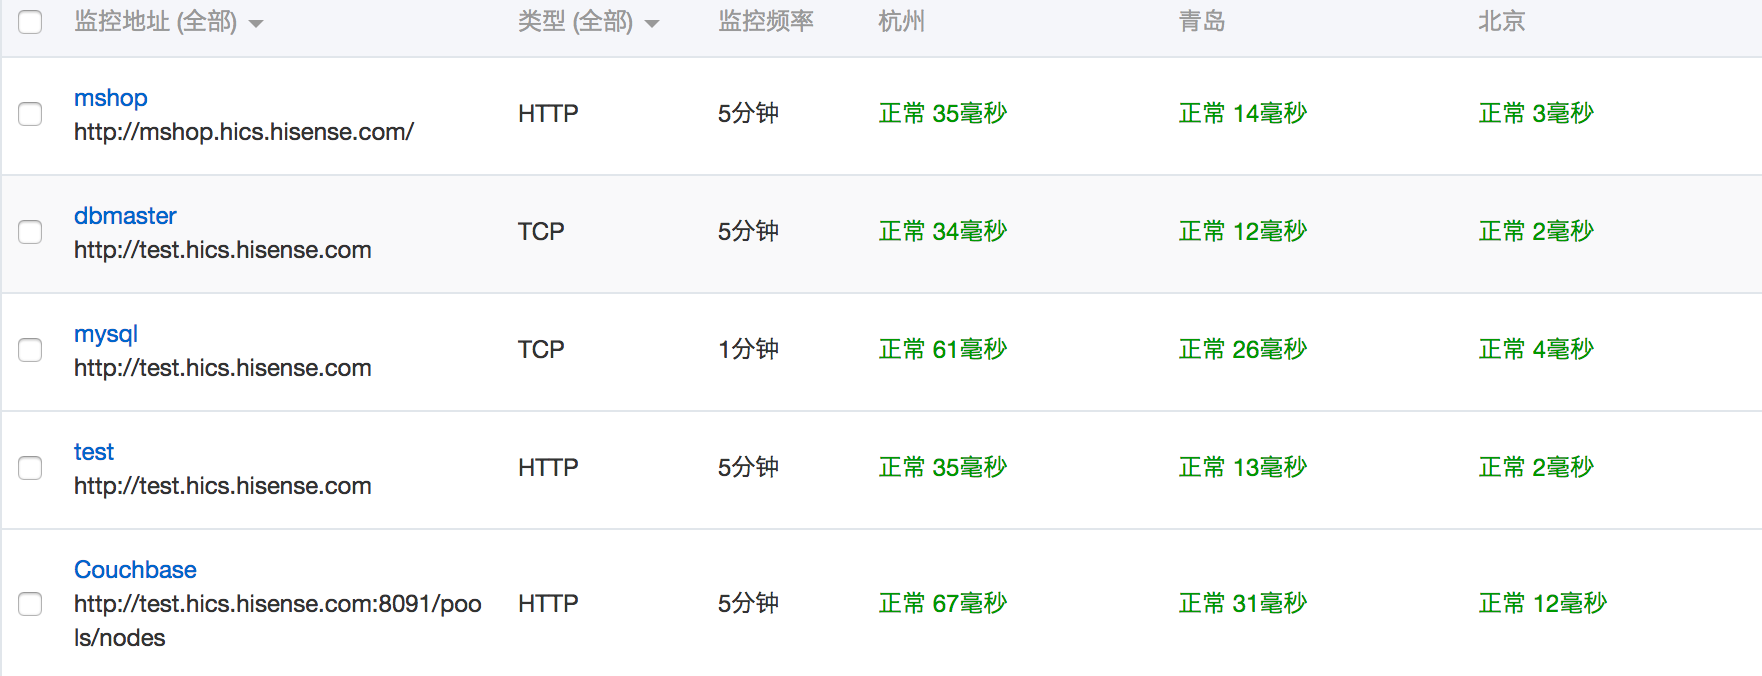
\includegraphics[width=6in]{chap05/aliyun1}
  \caption{站点监控状态图}
  \label{fig:aliyun1}
\end{figure}

\item 云服务器监控

云服务器的监控是指通过安装在服务器中的阿里云监控插件获取云服务器的状态,对于所有的云服务监控的规则都是一样的,均为CPU使用率、内存使用率和磁盘使用率三个方面,监控的具体规则如表~\ref{tab:aliyun-ecs}所示:
\begin{table}[H]
  \centering
  \begin{minipage}[t]{0.8\linewidth} % 如果想在表格中使用脚注,minipage是个不错的办法
  \caption[阿里云监控]{云服务器监控规则}
  \label{tab:aliyun-ecs}
    \begin{tabularx}{\linewidth}{lX}
      \toprule[1.5pt]
      {\heiti 监控项} & {\heiti 监控描述}\\\midrule[1pt]
        CPU使用率 & 5分钟 CPU使用率 平均值>85\% 则报警\\
        内存使用率 & 5分钟 内存使用率 最大值>95\% 则报警\\
        磁盘使用率 & 5分钟 磁盘使用率 平均值>70\% 则报警\\
      \bottomrule[1.5pt]
    \end{tabularx}
  \end{minipage}
\end{table}

\item 负载均衡监控

负载均衡主要是监控负载均衡内的各个服务器的监控状态以及负载均衡的带宽状态,当负载均衡出现异常时,可以通知报警联系人及时做出应对。
\begin{itemize}
\item 生产环境应用负载均衡监控规则
\begin{table}[H]
  \centering
  \begin{minipage}[t]{0.8\linewidth} % 如果想在表格中使用脚注,minipage是个不错的办法
  \caption[阿里云监控]{生产环境应用负载均衡监控规则}
  \label{tab:aliyun-slb1}
    \begin{tabularx}{\linewidth}{lX}
      \toprule[1.5pt]
      {\heiti 监控项} & {\heiti 监控描述}\\\midrule[1pt]
        流出带宽&5分钟 流出带宽 平均值>3M/s 则报警\\
        流入带宽&5分钟 流入带宽 平均值>3M/s 则报警\\
        后端异常ECS实例数&1分钟 后端异常ECS实例数 平均值>0个 则报警\\
      \bottomrule[1.5pt]
    \end{tabularx}
  \end{minipage}
\end{table}
\item 生产环境数据库负载均衡监控规则
\begin{table}[H]
  \centering
  \begin{minipage}[t]{0.8\linewidth} % 如果想在表格中使用脚注,minipage是个不错的办法
  \caption[阿里云监控]{生产环境数据库负载均衡监控规则}
  \label{tab:aliyun-slb2}
    \begin{tabularx}{\linewidth}{lX}
      \toprule[1.5pt]
      {\heiti 监控项} & {\heiti 监控描述}\\\midrule[1pt]
        后端健康ECS实例数&1分钟 后端健康ECS实例数 平均值<1个 则报警\\
      \bottomrule[1.5pt]
    \end{tabularx}
  \end{minipage}
\end{table}
\item 测试环境负载均衡监控规则
\begin{table}[H]
  \centering
  \begin{minipage}[t]{0.8\linewidth} % 如果想在表格中使用脚注,minipage是个不错的办法
  \caption[阿里云监控]{测试环境负载均衡监控规则}
  \label{tab:aliyun-slb3}
    \begin{tabularx}{\linewidth}{lX}
      \toprule[1.5pt]
      {\heiti 监控项} & {\heiti 监控描述}\\\midrule[1pt]
        流出带宽&5分钟 流出带宽 平均值>3M/s 则报警\\
        流入带宽&5分钟 流入带宽 平均值>3M/s 则报警\\
        后端异常ECS实例数&1分钟 后端异常ECS实例数 平均值>0个 则报警\\
      \bottomrule[1.5pt]
    \end{tabularx}
  \end{minipage}
\end{table}
\end{itemize}
\item CDN监控

CDN监控是指通过监控每一个域名的流量状态来判断应用的访问是否正常,当遇到DDos攻击时,CDN的流量会出现明显异常,通过监控这些异常,及时向运维人员报警,在很大程度上可以减少CDN流量的损失并降低被攻击的风险。

目前CDN监控的规则如表~\ref{tab:aliyun-cdn}所示:
\begin{table}[H]
  \centering
  \begin{minipage}[t]{0.8\linewidth} % 如果想在表格中使用脚注,minipage是个不错的办法
  \caption[阿里云监控]{CDN监控规则}
  \label{tab:aliyun-cdn}
    \begin{tabularx}{\linewidth}{lXX}
      \toprule[1.5pt]
      {\heiti 报警维度} & {\heiti 监控项} & {\heiti 监控描述}\\\midrule[1pt]
        fileserver&网络带宽峰值&5分钟 宽带峰值 平均值>4000000bit/s 则报警\\
        fileserver&公网下行流量&5分钟 公网网络出流量 求和值>100M/s 则报警\\
        img&网络带宽峰值&5分钟 宽带峰值 平均值>4000000bit/s 则报警\\
        web&网络带宽峰值&5分钟 宽带峰值 平均值>5000000bit/s 则报警\\
      \bottomrule[1.5pt]
    \end{tabularx}
  \end{minipage}
\end{table}
\end{enumerate}
\section{自定义服务监控}

虽然阿里云的云监控功能比较成熟,但是对于错误恢复和特殊需求的监控做的还相对不足,因此需要在本地的服务器中自己搭建监控环境,以提升系统的稳定性。

\subsection{心跳监听}

为了保证监控系统的高可用性,需要在APP1和APP2两个应用服务器内同时搭建监控系统,为了保证两套监控系统在同一时间只有一个监控系统在运行需要配置心跳监听,从监控节点通过心跳来监听主监控节点的运行状态,当主监控节点出现故障时,从监控节点运行监控进程,保证监控的正常\cite{巩天宁2012基于}。

Heartbeat是一款开源的提供高可用(Highly-Available)服务的软件,通过Heartbeat可以将资源(IP及程序服务等资源)从一台已经故障的计算机快速转移到另一台正常运转的机器上继续提供服务,称之为高可用服务。在实际生产应用场景中,heartbeat的功能和keepalived有很多相似之处,但在生产中,对实际的业务应用还是有区别的。如:keepalived主要是控制ip的漂移,配置、应用简单,而heartbeat则不但可以控制ip漂移,更擅长对资源服务的控制,配置、应用比较复杂~\cite{郭绪晶2012服务器集群系统高可用模块设计与实现}。由于Heartbeat能够对资源服务进行控制,所以本论文使用Heartbeat作为心跳监听的工具。

在服务器中配置心跳监听主要有以下步骤:
\begin{enumerate}
% \item 下载和安装Heartbeat软件

% 访问 http://www.linux-ha.org/wiki/Downloads 下载Heartbeat软件,解压完成后进入软件的目录中,执行以下命令完成安装:
% \begin{lstlisting}[language=sh,numbers=none]
% ./bootstrap
% #进入源码目录生成配置文件:
% ./ConfigureMe configure
% #编译安装
% make && make install
% \end{lstlisting}
% 安装完成后出现下面的信息表示安装成功:
% \begin{lstlisting}[numbers=none]
% heartbeat configuration:
%     Version                  = "3.0.6"
%     Executables              = "/usr/sbin"
%     Man pages                = "/usr/share/man"
%     Libraries                = "/usr/lib64"
%     Header files             = "/usr/include"
%     Arch-independent files   = "/usr/share"
%     Documentation files      = "/usr/share/doc/heartbeat"
%     State information        = "/var"
%     System configuration     = "/etc"
%     Init (rc) scripts        = "/etc/rc.d/init.d"
%     Init (rc) defaults       = "/etc/sysconfig"
%     Use system LTDL          = "yes"
%     HA group name            = "haclient"
%     HA group id              = "987"
%     HA user name             = "hacluster"
%     HA user user id          = "991"
%     Build dopd plugin        = "yes"
%     Enable times kludge      = "yes"
%     CC_WARNINGS              = " -Wall -Wmissing-prototypes -Wmissing-declarations -Wstrict-prototypes -Wdeclaration-after-statement -Wpointer-arith -Wwrite-strings -Wcast-qual -Wcast-align -Wbad-function-cast -Winline -Wmissing-format-attribute -Wformat=2 -Wformat-security -Wformat-nonliteral -Wno-long-long -Wno-strict-aliasing -Werror "
%     Mangled CFLAGS           = "-g -O2  -Wall -Wmissing-prototypes -Wmissing-declarations -Wstrict-prototypes -Wdeclaration-after-statement -Wpointer-arith -Wwrite-strings -Wcast-qual -Wcast-align -Wbad-function-cast -Winline -Wmissing-format-attribute -Wformat=2 -Wformat-security -Wformat-nonliteral -Wno-long-long -Wno-strict-aliasing -Werror  -ggdb3 -funsigned-char"
%     Libraries                = "-lbz2 -lz -lc -luuid -lrt -ldl  -lltdl"
%     RPATH enabled            = "no"
%     Distro-style RPMs        = "no"
% Note: If you use the 'make install' method for installation you
%     also need to adjust '/etc/passwd' and '/etc/group' manually.
% \end{lstlisting}
\item 配置Heartbeat软件,实现两个服务器的心跳监听

heartbeat 软件在使用时主要需要配置3个文件,分别是认证文件authkeys,配置文件ha.cf 和 资源文件haresources。authkeys主要配置节点之间的认证方式;ha.cf是主要的配置文件,配置节点信息、网络信息、监听频率等;haresources主要配置需要运行的程序或脚本。这里以app1/app2两节点为例,其IP分别是10.46.170.191/10.172.89.141,这里示例的配置文件为app1的,app2的参考app1配置即可。

ha.cf主配置文件配置项如表~\ref{tab:heartbeat}所示:
\begin{table}[H]
  \centering
  \begin{minipage}[t]{0.8\linewidth} % 如果想在表格中使用脚注,minipage是个不错的办法
  \caption[Heartbeat]{心跳监听主配置文件参数}
  \label{tab:heartbeat}
    \begin{tabularx}{\linewidth}{lXX}
      \toprule[1.5pt]
      {\heiti 参数项} & {\heiti 参数内容} & {\heiti 参数描述}\\\midrule[1pt]
      logfile  & /var/log/ha-log &  日志路径口\\
      keepalive  & 2 &  发送心跳报文的间隔,默认单位为秒 \\
      deadtime  & 30 & 认为对方宕掉的间隔时间 \\
      warntime & 10 &  认为对方可能宕掉的间隔时间\\
      initdead & 120 & 等待对方启动的最大时间\\
      udpport & 694 & 表示heartbeat广播/单播通讯使用的udp端口\\
      bcast & eth0 & 心跳所使用的网络接口\\
      ucast & eth0 10.172.89.141 & 单播通讯,对方网络接口及IP地址\\
      auto\_failback & on & 表示当主节点正常之后是否将资源/服务切换回来\\
      node & app1,app2 & 就是heartbeat集群中的节点信息 \\
      \bottomrule[1.5pt]
    \end{tabularx}
  \end{minipage}
\end{table}
% \begin{lstlisting}[numbers=none]
% # 日志路径
% logfile /var/log/ha-log
% # 发送心跳报文的间隔,默认单位为秒。
% keepalive 2
% # 认为对方宕掉的间隔时间。
% deadtime 30
% # 认为对方可能宕掉的间隔时间。
% warntime 10
% # 等待对方启动的最大时间。
% initdead 120
% # 表示heartbeat广播/单播通讯使用的udp端口。
% udpport 694
% # 心跳所使用的网络接口。
% bcast   eth0
% # 单播通讯,对方网络接口及IP地址。
% ucast eth0 10.172.89.141
% # 表示当主节点正常之后是否将资源/服务切换回来。
% auto_failback on
% # 就是heartbeat集群中的节点信息。
% node    app2
% node    app1
% \end{lstlisting}
在配置过程中将app1配置为主节点,当配置auto\_failback为off时,app1节点异常时app2会接管继续执行监控程序,app1节点恢复后也不会移交监控程序,当配置auto\_failback为on时,app1节点恢复后app2会将资源移交回app1.

authkeys主配置文件配置如下:
\begin{lstlisting}[numbers=none]
auth 2
#1 crc
2 sha1 mimaminishop
#3 md5 somewords
\end{lstlisting}
此文件为不同集群中 heartbeat 节点进行连接的认证文件, 不同集群中该文件采用的算法和密钥必须相同,认证方式有 3 种算法:crc方式、md5加密方式和sha1哈希方式。三种方式中 crc方式只能够校验节点间通信的校验数据包是否损坏,不能进行安全性认证; sha1/md5 两种方式需要进行安全性认证,它们通过一个密钥来进行认证。sha1和md5两种方式相比,sh1方式的资源消耗远小于md5方式,因此在大多数应用中建议使用 sha1 方式\cite{heartbeat配置说明}。

可以看出,示例中使用的是sha1算法,如果要换用其他算法只需要修改auth指令后面的数字,然后取消相应行的注释即可。另外,该文件的属性必须为600,否则heartbeat启动将失败。

haresources主配置文件配置如下:
\begin{lstlisting}[numbers=none]
app1 system_monitor
\end{lstlisting}
这表示Heartbeat启动时会执行资源路径中的system\_monitor脚本,实现服务的监控。

\item 配置监控脚本,实现服务的监控。

目前系统服务的监控主要包括系统服务状态的监控和系统数据库状态的监控,通过Heartbeat可以保证上述监控的高可用性;首先开发系统的监控脚本system\_monitor脚本,脚本的具体内容参见附录~\ref{cha:systemmonitor},通过脚本的内容可以看出在保证监控程序高可用的情况下,在监控频率上也进行相应的配置,将监控的频率设置为30s,表示监控程序每30秒会对所有的服务状态和数据库状态进行一次轮询检查,出现异常进行相应的处理,大大保证了监控的有效性。

监控脚本的主要流程和策略可以参见图~\ref{fig:systemmonitor},服务的监控主要是对Tomcat服务和MySQL服务的运行状态进行监控,数据库状态的监控主要是对数据库的主从同步状态进行监控,确保数据的完整性。
\begin{figure}[H] % use float package if you want it here
  \centering
  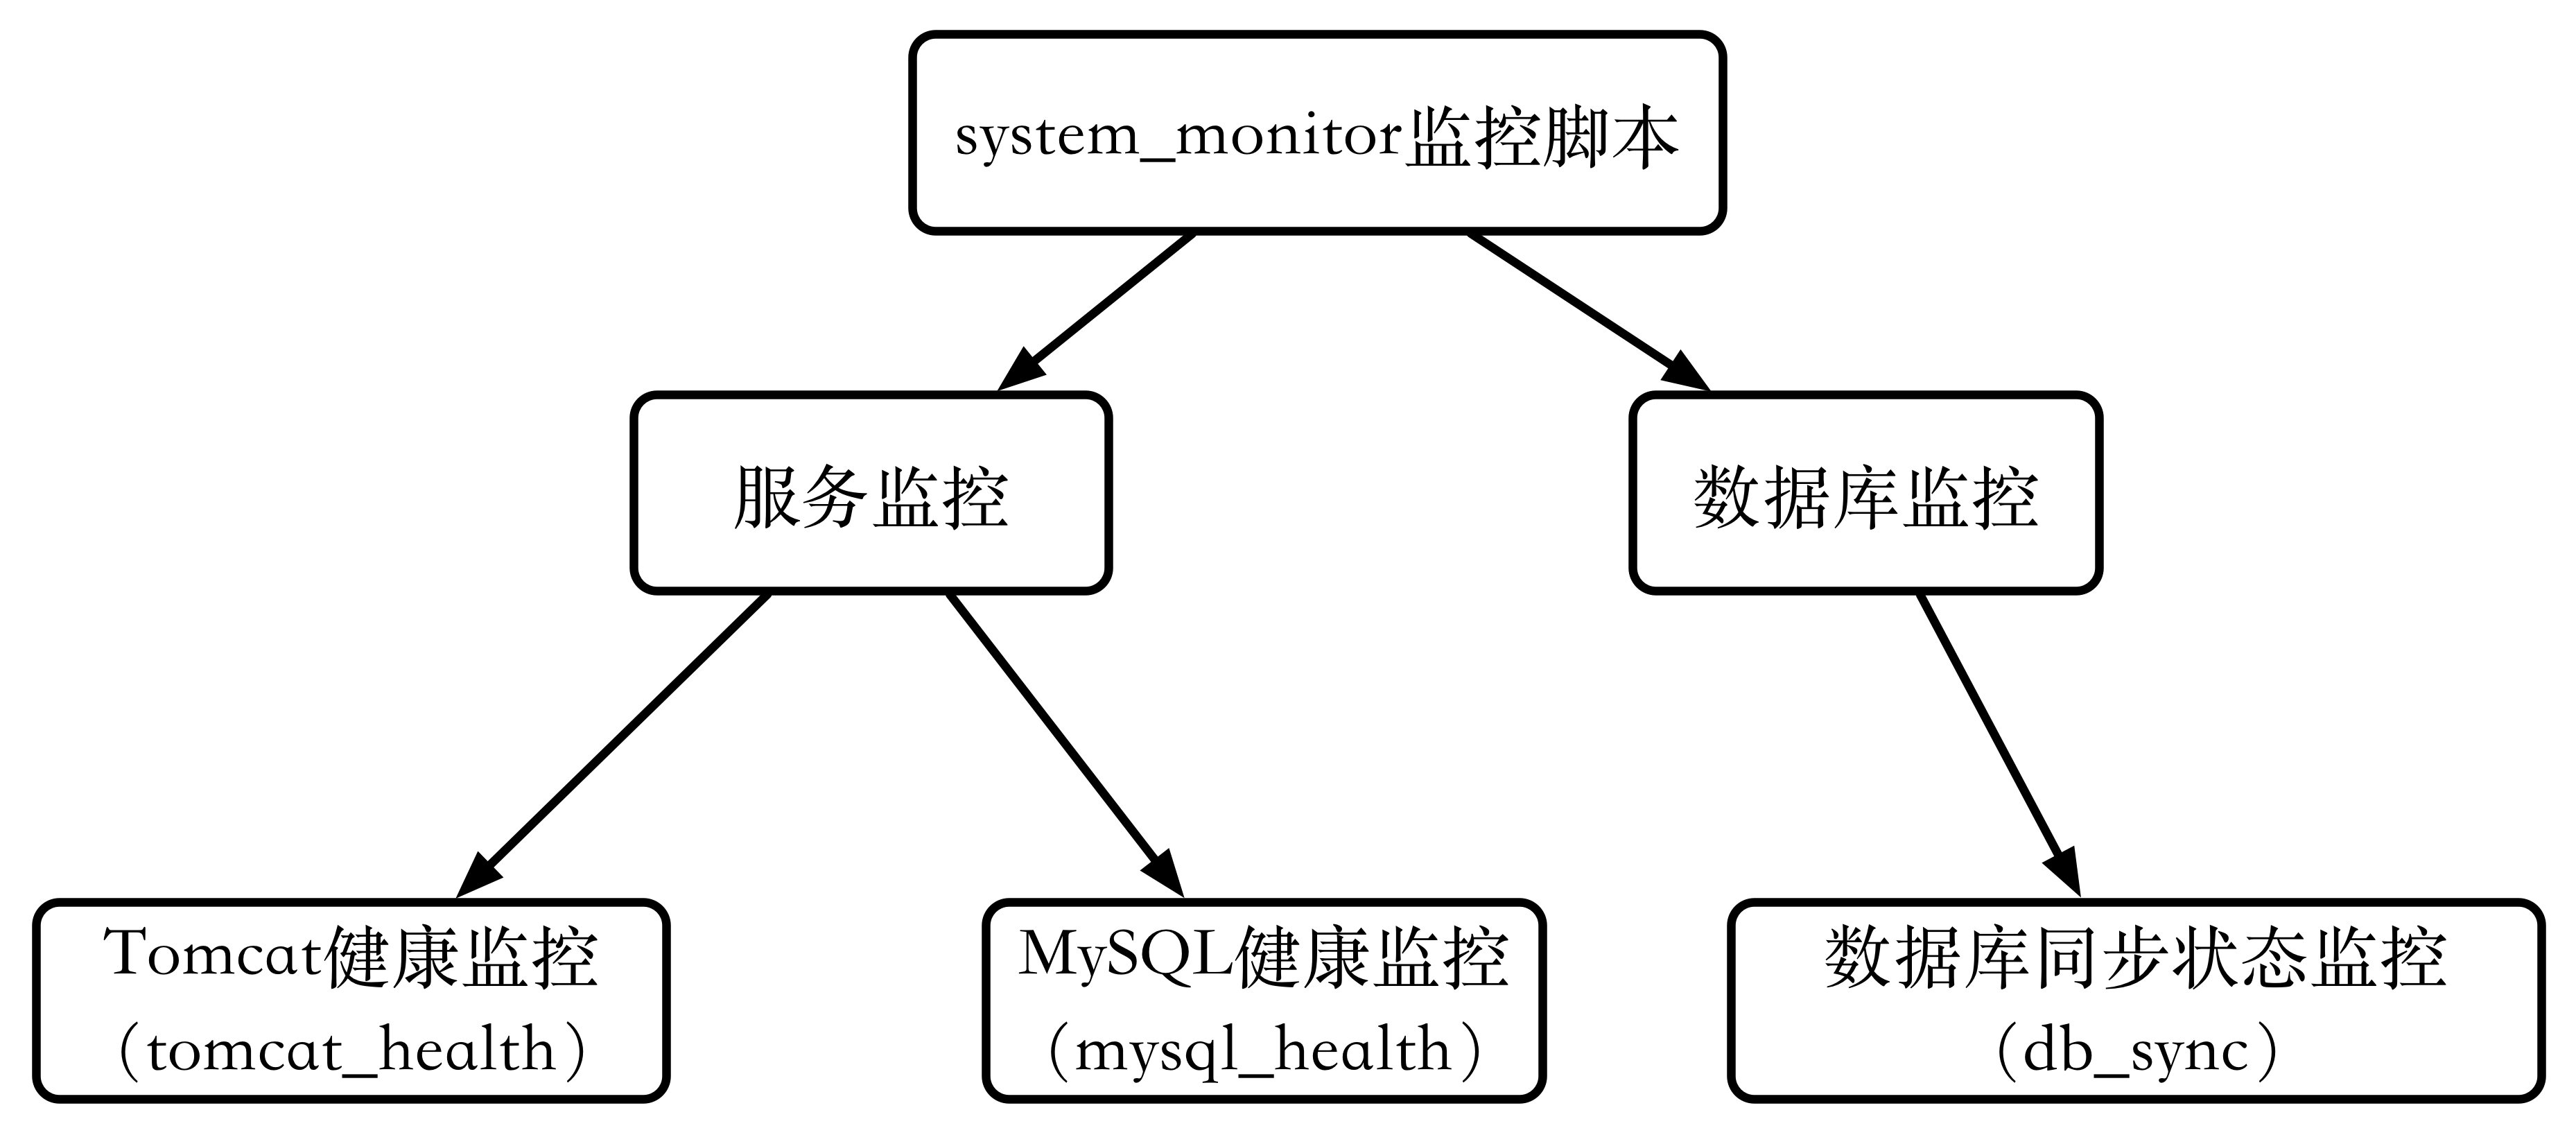
\includegraphics[width=5in]{chap05/monitor}
  \caption{系统监控方案}
  \label{fig:systemmonitor}
\end{figure}

监控脚本设计和开发完成后,通过在app1和app2两台服务器上同时部署监控脚本,这样在app1服务器出现故障的情况下,app2会获得app1故障的消息,自身启动监控脚本确保监控的正常运行。由于在上一部分我们在配置心跳监听时,将auto\_failback参数配置为on,这表示当app1服务器状态恢复正常后,app2会主动停止自身的监控程序,将监控程序移交给app1服务器,这样既保证了监控的正常运行也实现了监控的高可用。

通过system\_monitor脚本,每30秒对脚本中的监控服务进行一次监听,如果有新的监控脚本,可以在该脚本中配置其他脚本的路径并完成相关配置。
\end{enumerate}

\subsection{Tomcat监控方案设计}
Tomcat是应用运行的容器,要保证WEB应用的正常运行必须要先保证Tomcat服务的正常运行,正常情况下我们在小型项目的开发过程中可以通过访问服务器,执行CentOS系统自带的服务状态命令查看Tomcat服务的状态:
\begin{lstlisting}[numbers=none]
systemctl status tomcat
\end{lstlisting}
执行上述命令后,终端中会显示tomcat服务的运行状态情况,如图~\ref{fig:tomcatmonitor}所示:
\begin{figure}[H] % use float package if you want it here
  \centering
  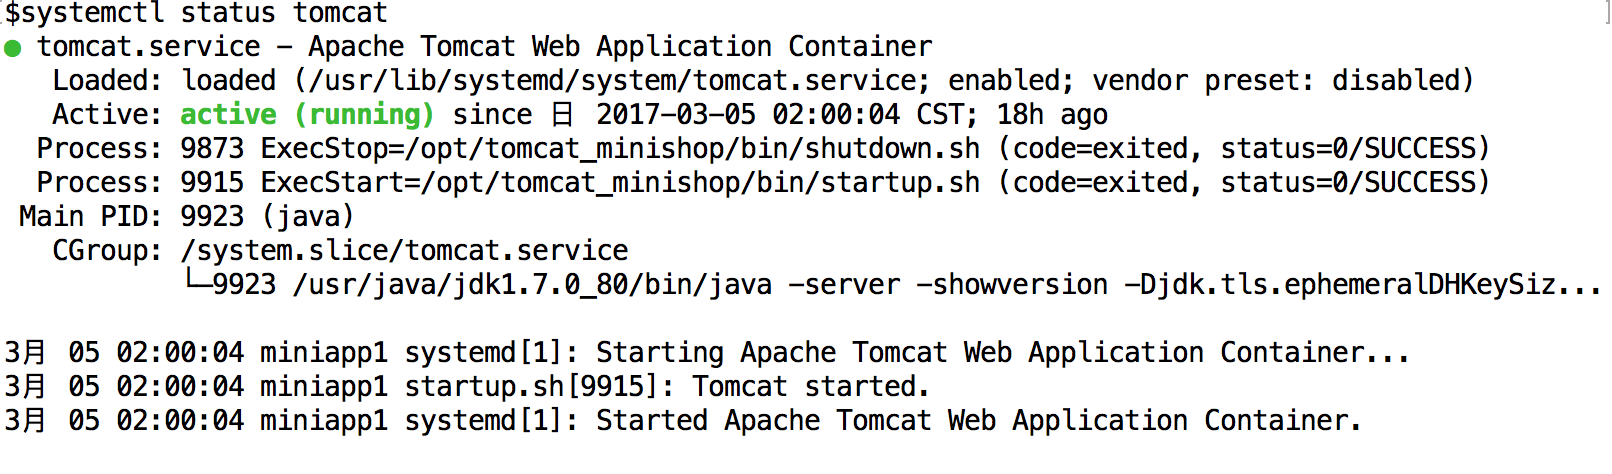
\includegraphics[width=5in]{chap05/tomcat}
  \caption{tomcat服务状态}
  \label{fig:tomcatmonitor}
\end{figure}
active(running)表示服务正常运行,除此之外还有其他的几种状态如表~\ref{tab:tomcat-status}所示:

\begin{table}[htb]
  \centering
  \begin{minipage}[t]{0.8\linewidth} % 如果想在表格中使用脚注,minipage是个不错的办法
  \caption[Tomcat]{Tocmat状态}
  \label{tab:tomcat-status}
    \begin{tabularx}{\linewidth}{lX}
      \toprule[1.5pt]
      {\heiti 状态} & {\heiti 描述}\\\midrule[1pt]
      active  &  运行正常  \\
      failed  &  启动失败  \\
      unknown &  未知错误\\
      \bottomrule[1.5pt]
    \end{tabularx}
  \end{minipage}
\end{table}

为了实现对于Tocmat的远程监控以及脚本监控,我们需要根据以上的几种运行状态去设计监控过程中对于Tomcat运行状态的判断和故障通知,除此之外,还需要使用可以通过SSH协议执行远程命令的Python库来实现在第三方服务器上开发Tomcat状态监控和通知的脚本。

综上,本论文选择Python的ssh库实现对于远程服务的ssh访问,通过ssh库中SSHClient()对象的connect方法可以建立本地对于远程服务器的连接,建立连接之后我们就可以执行远程命令了,这一部分同样通过ssh库的exec\_command函数来实现,通过该函数在被监控服务器端执行systemctl is-active tomcat.service命令来监测Tomcat服务的健康状态,根据不同的服务运行状态设计Python脚本返回的服务运行状态码,如表~\ref{tab:tomcat-code}所示:
\begin{table}[htb]
  \centering
  \begin{minipage}[t]{0.8\linewidth} % 如果想在表格中使用脚注,minipage是个不错的办法
  \caption[Tomcat]{自定义返回状态码}
  \label{tab:tomcat-code}
    \begin{tabularx}{\linewidth}{lX}
      \toprule[1.5pt]
      {\heiti 状态码} & {\heiti 描述}\\\midrule[1pt]
      100  &  表示WEB访问正常  \\
      101  &  表示WEB应用异常,需要查看日志  \\
      102  &  Tomcat服务停止,需要重启  \\
      103  &  服务不存在,需要查看日志\\
      104  &  服务器连接失败,需要查看是网络问题还是服务器异常  \\
      105  &  服务重启  \\
      106  &  其他异常\\
      200  &  重启成功  \\
      201  &  重启失败  \\
      \bottomrule[1.5pt]
    \end{tabularx}
  \end{minipage}
\end{table}

在Python监控脚本中,如果出现可以自动解决的问题比如服务停止的异常,可以通过执行远程命令systemctl restart tomcat.service命令来重新启动Tomcat服务,最终Python监控脚本将状态码返回到SHELL监控脚本中。

以上提到的Python监控脚本仅仅是对于Tomcat状态监控的脚本,在实际应用中除了状态监控以外我们还需要考虑到日志存储和短信通知的问题,这些问题我们通过设计一个shell监控脚本来实现日志记录和短信通知的功能。首先我们通过调用Python监控脚本,根据脚本返回的状态码来进行判断,然后根据判断结果进行日志的记录和短信通知。

综合上述介绍的两部分,Tomcat监控的框架可以描述为图~\ref{fig:tomcat-frame}所示:
\begin{figure}[H] % use float package if you want it here
  \centering
  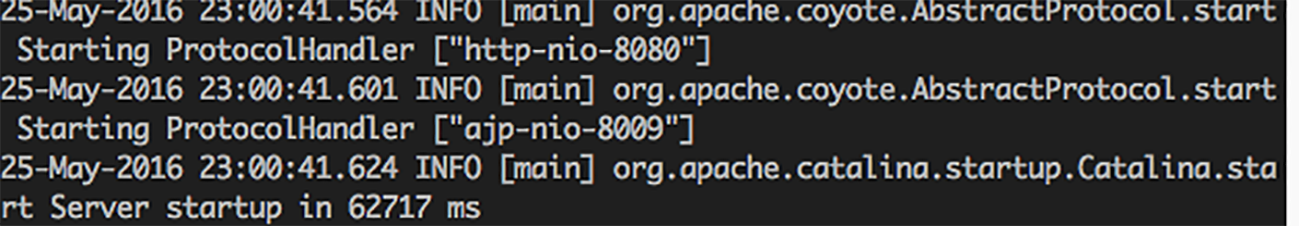
\includegraphics[width=5in]{chap05/tomcat2}
  \caption{Tomcat监控框架}
  \label{fig:tomcat-frame}
\end{figure}

具体的监控和故障处理脚本可以通过附录~\ref{cha:Tomcathealth}和附录~\ref{cha:Tomcatfailover}来查看。
\subsection{数据库监控方案设计}

除了WEB应用容器Tomcat容器的监控,对数据库的监控对于系统的稳定性来说也是非常重要的,为了最大程度的保证数据库的稳定性和数据的完整性,本论文对于数据库部分设计开发了相对应的监控方案,为了保证数据库服务的正常运行设计开发了数据库健康状态监控方案;为了保证数据的完整性和高可用性设计开发了主从数据库复制状态监控。

\begin{enumerate}
\item 数据库健康状态监控方案

对于数据库的健康状态监控,可以通过跟Tomcat监控方案类似的方法进行监控,但是考虑到执行SSH命令对于系统的安全性来说有一定程度的威胁,而且MySQL服务本身可以实现远程的连接与访问,因此本部分没有使用基于SSH协议的远程命令执行方案对数据库健康状态进行监控,而是采用执行本地mysql命令访问远程的数据库,通过执行sql语句的命令来实现数据库健康状态监控。这样做的优势在于"systemctl status " 命令可以判断MySQL服务是否正常运行,且执行效率高。缺点在于无法检查MySQL内部异常导致服务异常但是运行正常的现象。

对于MySQL而言,其自身的"show status"命令可以获取到MySQL运行时的相关参数,包括进程状态、连接状态、存储引擎状态等相关信息,通过对有效参数进行判断可以准确的获取MySQL的健康状态,如果有正常的数据返回则说明数据库运行正常,否则数据库的健康状态出现问题。当出现问题时,首先需要通知运维人员,为了实现通知功能本论文开发了短信通知的功能,这部分可以参考下一节,其次需要对当前的问题进行分析和判断,如果主从两台服务器的数据库的健康状态均出现问题,那么只能通过通知运维人员以人工介入的方式来解决问题,如果只有一台服务器的数据库健康状态出现问题,那么需要通过调整数据库负载均衡,将出现问题的数据库的权重设置为0,正常的数据库权重设置为100,保证数据库服务的正常运行,然后尝试重启异常的数据库服务进行故障恢复。

为了实现数据库负载均衡的动态调整,需要开发针对于阿里云负载均衡的权重调整脚本,通过分析和使用阿里云的负载均衡SDK来开发权重调整脚本,通过SDK的DescribeLoadBalancerAttributeRequest包来获取当前数据库负载均衡的状态,通过SetBackendServersRequest对负载均衡的权重进行调整,最终返回权重调整的结果。

为了实现数据库服务的远程重启,需要开发针对于Docker API的容器启动脚本,通过docker SDK的Client方法同远程服务器进行连接,通过inspect\_container方法获取远程容器的运行状态,如果MySQL容器的状态异常则通过restart方法进行重启。

综上所述,数据健康监控脚本的执行流程和顺序如图~\ref{fig:mysql-healty-monitor}所示。
\begin{figure}[H] % use float package if you want it here
  \centering
  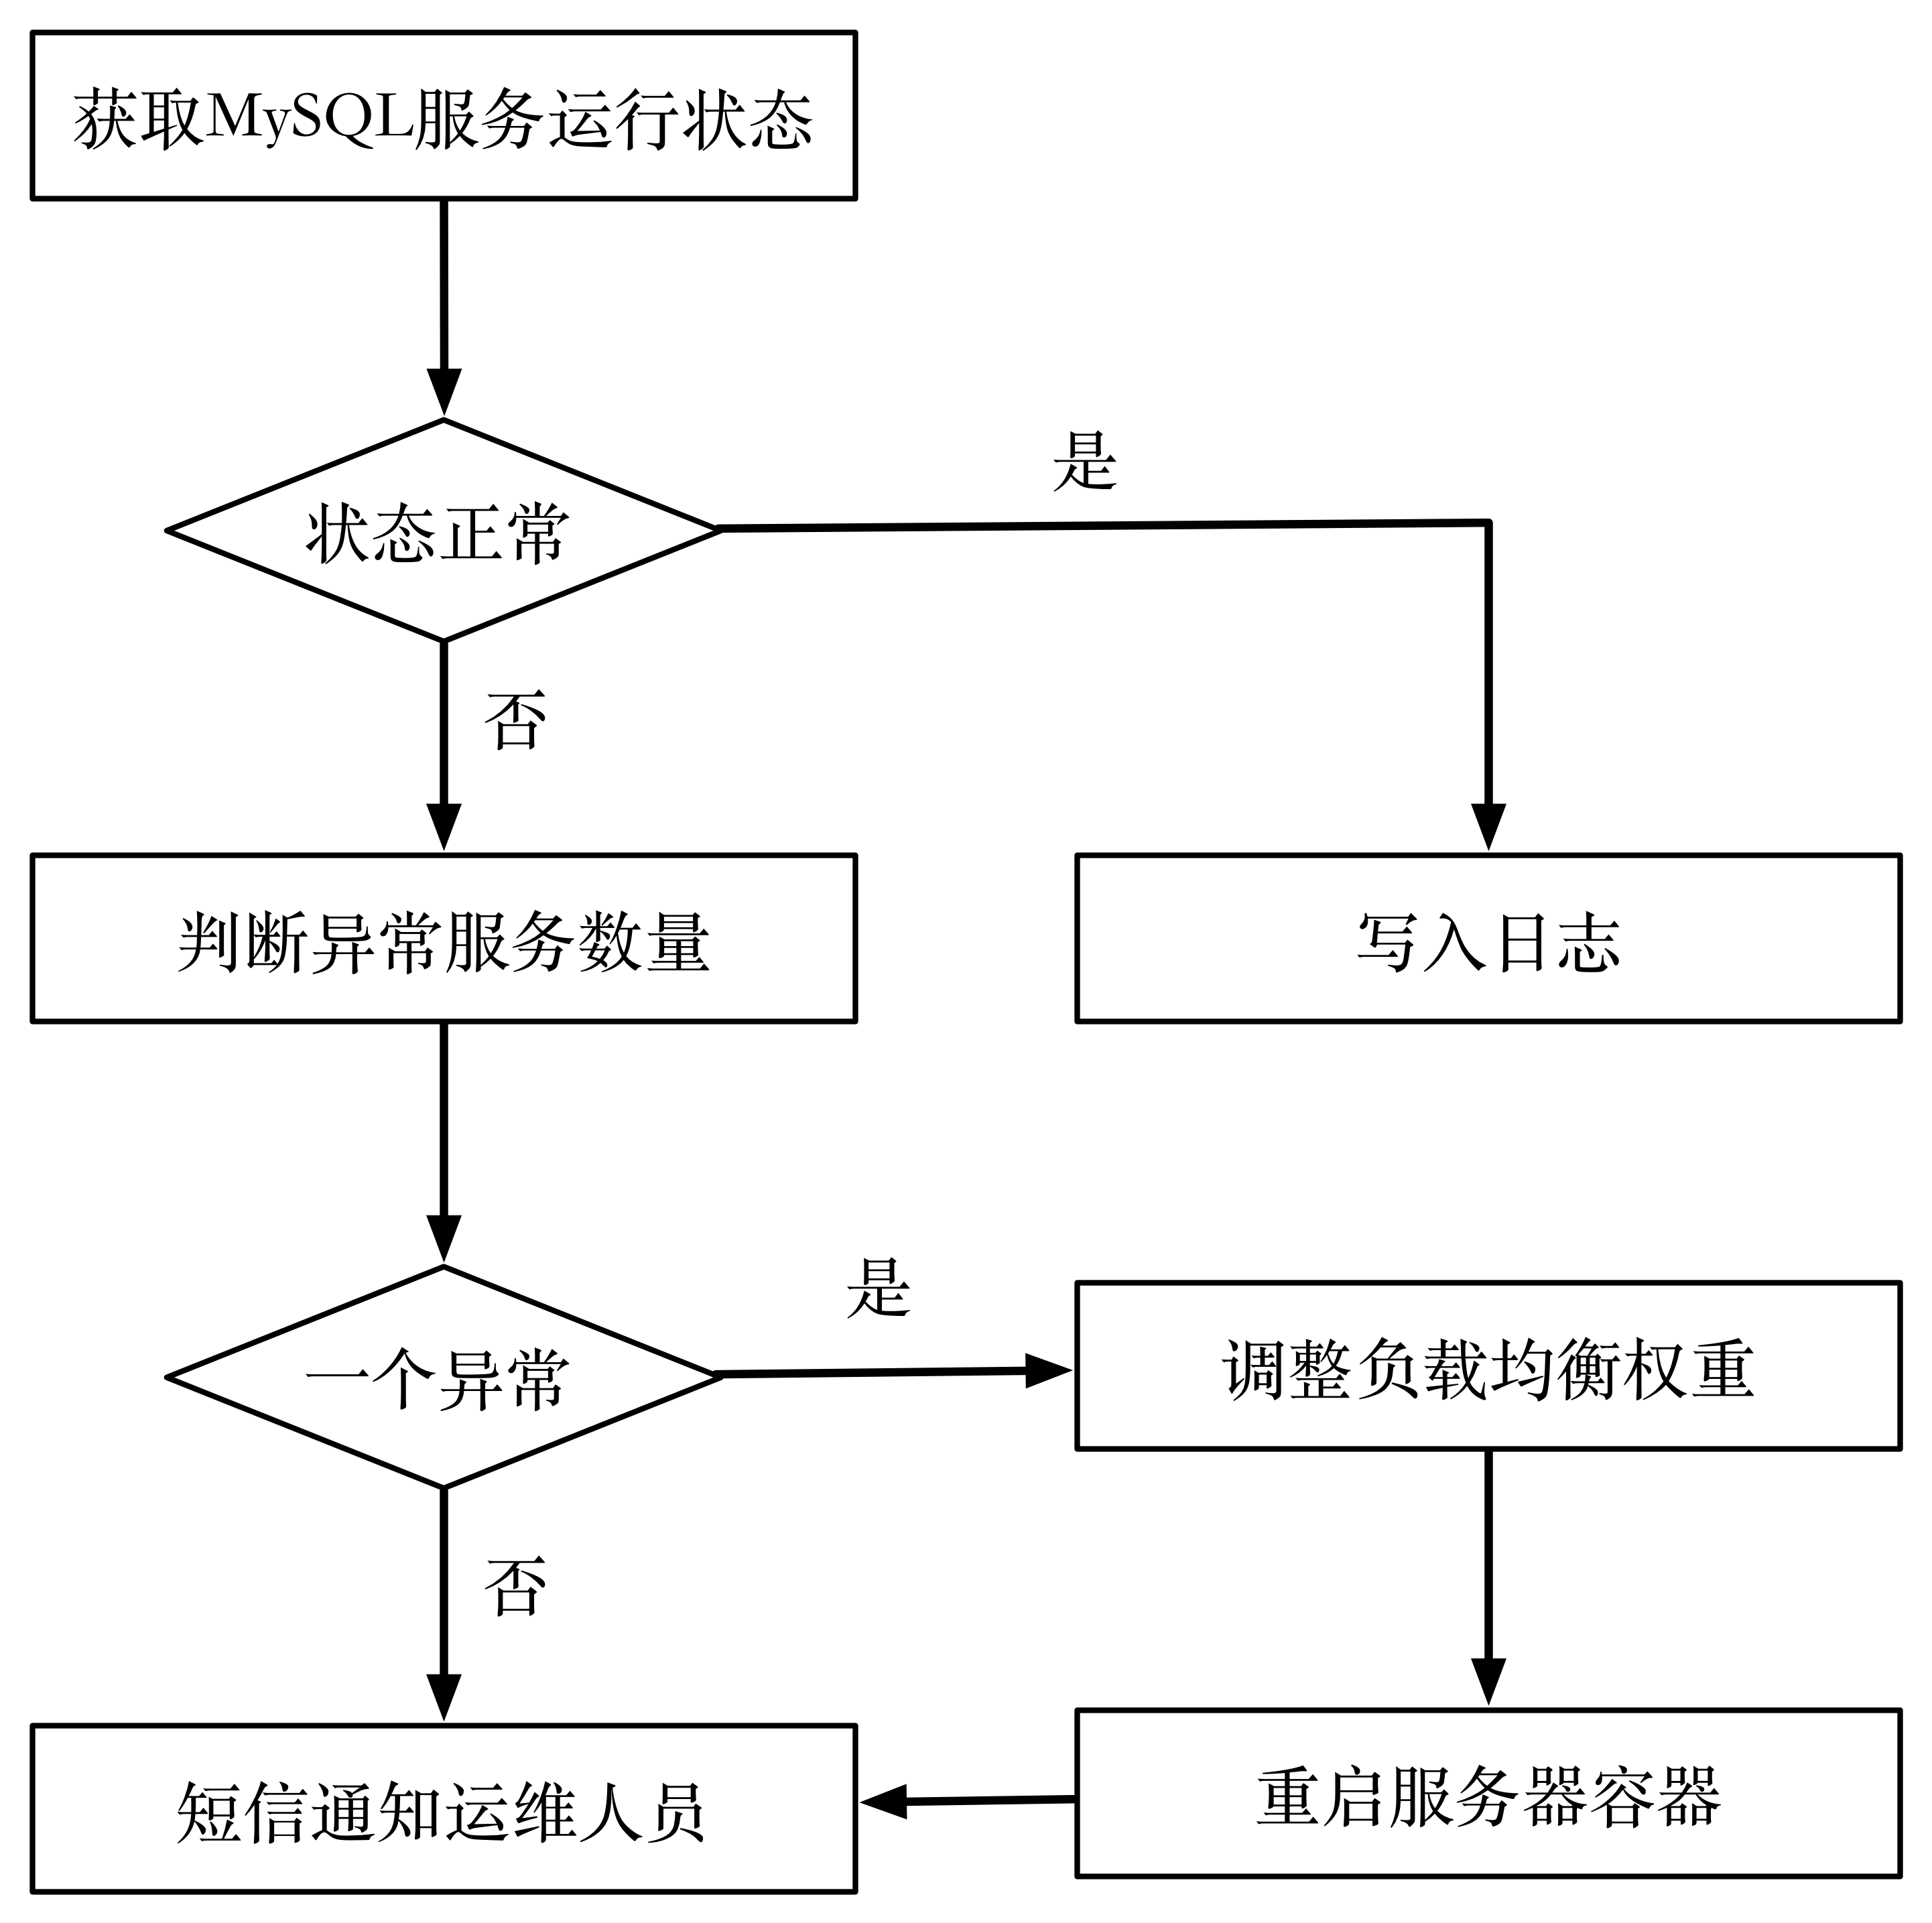
\includegraphics[width=5in]{chap05/mysql1}
  \caption{数据库健康状态监控方案}
  \label{fig:mysql-healty-monitor}
\end{figure}
完整的数据库健康监控脚本可以参考附录~\ref{cha:mysqlhealth}。

\item 数据库主从复制状态监控方案

针对数据库的主从数据库复制的问题性和数据一致性的问题,需要设计数据库主从复制状态监控方案,方案的目的就是通过执行主从复制的sql语句show slave status来获取数据库主从复制的状态,根据返回的参数值判断数据主从复制是否正常,如果正常则记录正常日志,否则需要将错误信息记录到日志文件中并短信通知运维人员。

对于执行show slave status语句后返回的数据库主从复制状态参数,主要通过以下三个方面判断数据库状态是否正常:
\begin{itemize}
  \item 通过Slave\_IO\_Running和Slave\_SQL\_Running两个参数的值来判断从库的复制状态是否正常,第一个参数负责与主机IO通信,第二个参数负责自己的slave mysql进程,如果两个参数的值均为YES则说明从库复制状态正常,否则说明复制状态不正常,需要检查从库的日志来进行问题的定位。这是进行数据库复制状态检查的第一步,只有以上两个参数值均为YES时才会进行下面的判断,否则直接将错误信息写入日志并短信通知运维人员。
  \item 通过Seconds\_Behind\_Master参数的值来判断主从复制的延迟,如果延迟时间大于300毫秒则说明主从复制状态异常,需要记录错误信息并短信通知运维人员,否则说明复制状态正常,需要进行下一步的判断。
  \item 通过Master\_Log\_File,Relay\_Master\_Log\_File,Read\_master\_log\_Pos和Exec\_Master\_log\_pos四个参数的值来判断主从复制的最终状态,其中Master\_Log\_File表示主库的数据库当前写入的日志文件,Relay\_Master\_Log\_File表示从库读取到的主库日志文件,如果两个参数一致则表示日志文件正常;Read\_master\_log\_Pos表示当前主库操作的日志位置,Exec\_Master\_log\_pos表示当前从库执行的主库日志位置,如果这两个参数一致则表示从库执行的最新操作是主库的最后操作,不存在延迟情况,只有当以上两种情况同时正常时,才会最终确认数据库主从复制正常,否则会将错误信息记录到日志文件中,并通知运维人员人工干预修复异常。
\end{itemize}

数据库主从复制状态监控的流程如图~\ref{fig:mysql-sync-monitor}所示。
\begin{figure}[H] % use float package if you want it here
  \centering
  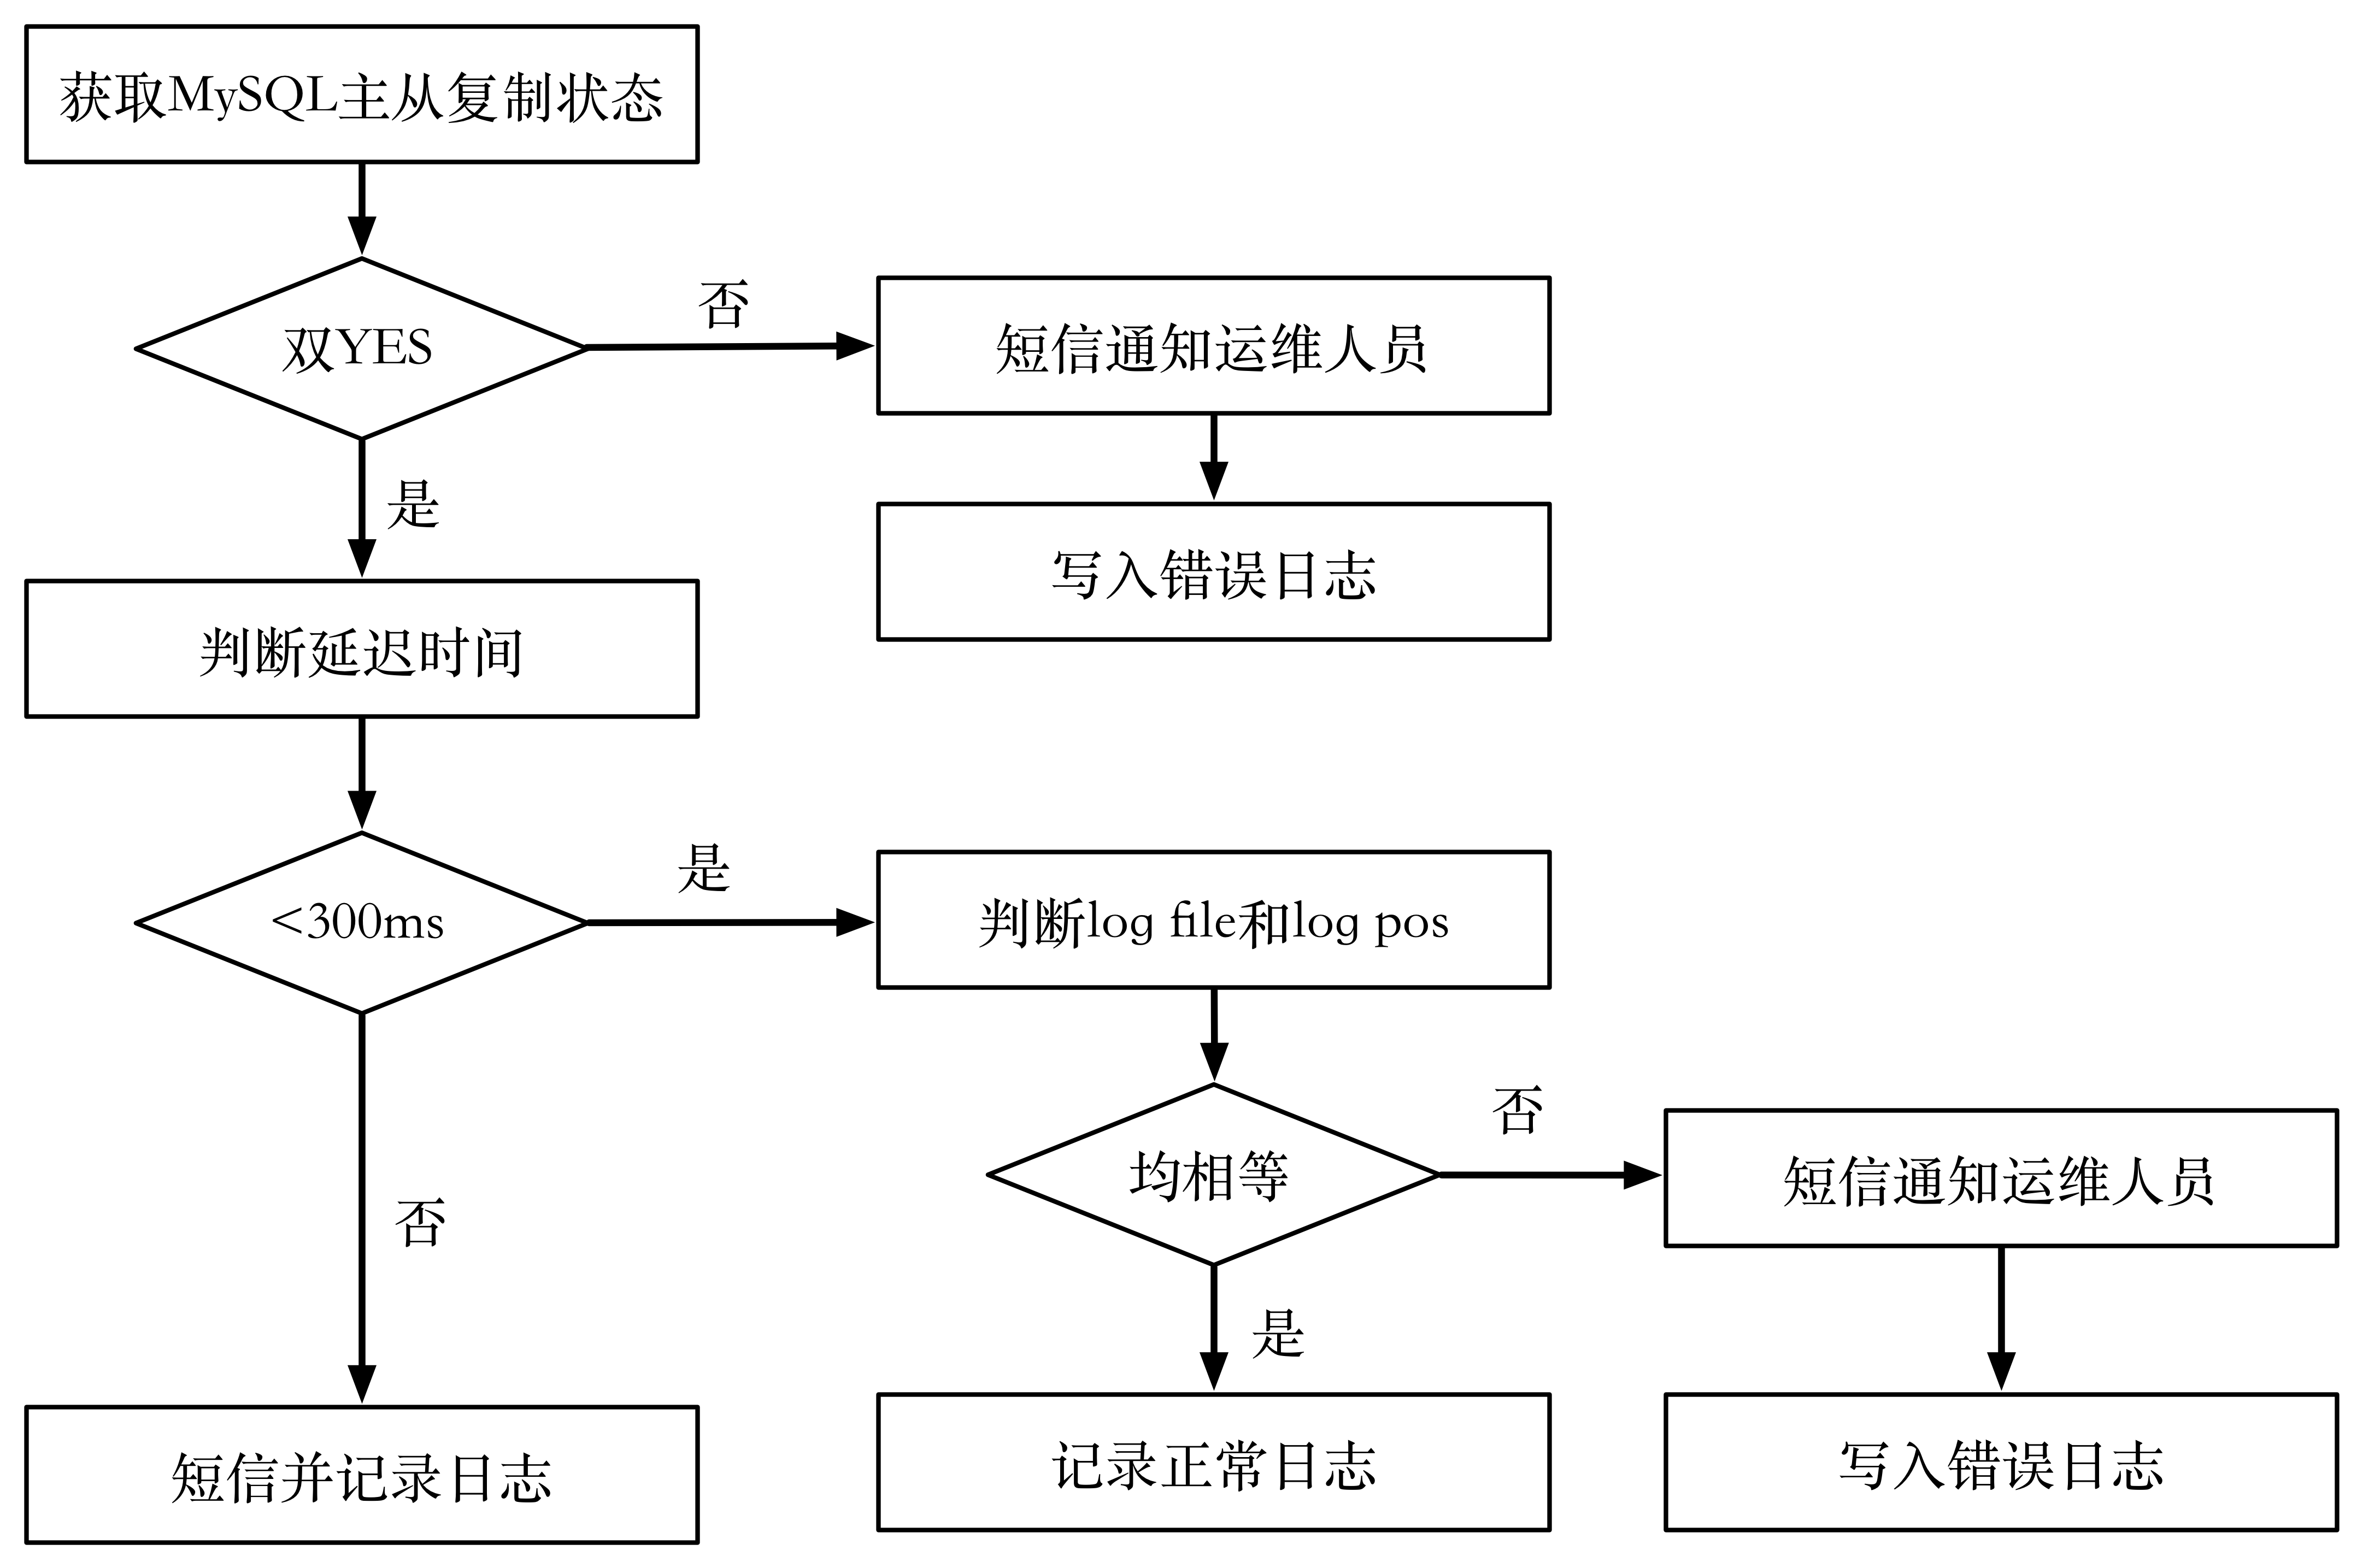
\includegraphics[width=5in]{chap05/mysql2}
  \caption{数据库主从复制状态监控方案}
  \label{fig:mysql-sync-monitor}
\end{figure}
数据库同步状态监控的脚本可以参考~\ref{cha:mysqlsync}。
\end{enumerate}

\section{短信通知方案设计}

在以前,当服务出现问题时无法及时的通知到运维人员,直到运维人员巡检或者应用的访问出现问题时运维人员才会发现故障,而现在有了监控的脚本,那么如何在第一时间通知运维人员就是需要解决的一大难题。通知时效性最高的就是短信通知,因此在服务器中开发一个能够发送短信的程序就显得非常重要\cite{陈泰伟2007基于短信平台的服务器监控系统关键技术探讨}。

为了实现短信的发送,首先需要选择和注册一个短信平台,因现有的云通讯平台短信发送的时间低于五秒,且支持自定义短信模版和支持API的特点,本论文选择云通讯作为系统的短信发送应用。

其次,需要在服务中安装SDK,同时开发短信发送脚本调用SDK以实现短信的发送,短信通知的脚本参考附录~\ref{cha:sms}。

在脚本中,首先需要根据自己注册的账户获取账户ID和验证Token,然后获取自己创建的应用的ID,完成基础的配置和认证。
在执行脚本时,通过SendTemplateSMS.py phone tempID content命令来发送短信,其中phone为接受短信的一个或者一组手机号,tempID为自己设计的短信模版对应的ID,contenet为短信的发送内容。

\section{日志备份方案设计}

在Tomcat的运行过程中,随着用户的访问,每天都会产生大量的访问日志和请求日志,随着时间的增加,日志的数量和空间占用会越来越大,为了解决日志的空间占用但又需要保证日志的存储以便后期进行日志分析的问题,需要设计开发日志备份脚本。主要的需求为:
\begin{itemize}
\item 每个月的1号会压缩上一个月的日志文件到压缩文件中
\item 每个月清理超过三个月的日志
\item 每个月压缩的日志上传到阿里云归档存储中进行备份
\end{itemize}
针对以上需求,开发的归档存储上传脚本参考附录~\ref{cha:aliyun-oas}。

通过oas库中oas\_api方法链接获取到OAS对象,通过对象的upload\_archive方法上传备份的日志文件。

开发的日志备份脚本可以参考附录~\ref{cha:Tomcatlog},脚本中首先通过匹配不同类型的日志名称来将日志文件分类压缩,然后通过执行OAS上传脚本上传压缩后的日志文件,上传完成后删除未压缩的日志文件。

日志备份脚本开发完成后,为了保证脚本每个月运行一次,需要修改crontab的配置文件,增加:
\begin{lstlisting}[numbers=none]
0 3 1 * * /opt/sh/Prod_tomcat_log_bak.sh
\end{lstlisting}
设置脚本执行时间为每个月1号的凌晨3点。
%\section{DockerAPI操作}
%\section{阿里云API优化}
\label{cha:Monitor-aliyun}
\section{本章总结}
本章主要对服务器层级的服务器监控措施和应急措施的优化策略研究,主要包括基于阿里云平台的自有监控和通知方案设计、个人开发的服务监控方案设计、短信通知脚本开发以及日志定期备份脚本开发等内容,通过以上的监控和优化措施,在最大程度上保证服务器和服务的正常运行、服务故障的自动恢复以及服务故障的通知,降低运维人员的时间成本,提升系统的稳定性。